%	草稿练习
\documentclass[hyperref]{ctexart}
\usepackage[left=2.50cm, right=2.50cm, top=2.50cm, bottom=2.50cm]{geometry} %页边距
\usepackage{helvet}
\usepackage{amsmath, amsfonts, amssymb} % 数学公式、符号
\usepackage[english]{babel}
\usepackage{graphicx}   % 图片
\usepackage{url}        % 超链接
\usepackage{bm}         % 加粗方程字体
\usepackage{multirow}
\usepackage{booktabs}
\usepackage{algorithm}
\usepackage{algorithmic}
\usepackage{cite}
\bibliographystyle{IEEEtran}
\graphicspath{{figures/}}
% Copyright 20120 Liutao Tian, MIT License
% https://github.com/andy123t/code-latex-style/

\usepackage{listings,color}

% Matlab highlight color settings
%\definecolor{mBasic}{RGB}{248,248,242}       % default
\definecolor{mKeyword}{RGB}{0,0,255}          % bule
\definecolor{mString}{RGB}{160,32,240}        % purple
\definecolor{mComment}{RGB}{34,139,34}        % green
\definecolor{mBackground}{RGB}{245,245,245}   % lightgrey
\definecolor{mNumber}{RGB}{134,145,148}       % gray

\definecolor{Numberbg}{RGB}{237,240,241}     % lightgrey

% Python highlight color settings
%\definecolor{pBasic}{RGB}{248, 248, 242}     % default
\definecolor{pKeyword}{RGB}{228,0,128}        % magenta
\definecolor{pString}{RGB}{148,0,209}         % purple
\definecolor{pComment}{RGB}{117,113,94}       % gray
\definecolor{pIdentifier}{RGB}{166, 226, 46}  %
\definecolor{pBackground}{RGB}{245,245,245}   % lightgrey
\definecolor{pNumber}{RGB}{134,145,148}       % gray

\lstnewenvironment{Python}[1]{
	\lstset{language=python,               % choose the language of the code
		xleftmargin=30pt,
		xrightmargin=10pt,
		frame=l,
		framesep=15pt,%framerule=0pt,  % sets the frame style
		%frame=shadowbox,rulesepcolor=\color{red!20!green!20!blue!20},
		%basicstyle=\small\ttfamily,          % sets font style for the code
		basicstyle=\footnotesize\fontspec{Consolas},
		keywordstyle=\color{pKeyword},       % sets color for keywords
		stringstyle=\color{pString},         % sets color for strings
		commentstyle=\color{pComment},       % sets color for comments
		backgroundcolor=\color{pBackground}, % choose the background color
		title=#1,                            %\lstname show the filename of files
		emph={format_string,eff_ana_bf,permute,eff_ana_btr},
		emphstyle=\color{pIdentifier}
		showspaces=false,                    % show spaces adding particular underscores
		showstringspaces=false,              % underline spaces within strings
		showtabs=false,                      % show tabs within strings adding particular underscores
		tabsize=4,                           % sets default tabsize to 2 spaces
		captionpos=t,                        % sets the caption-position to bottom
		breaklines=true,                     % sets automatic line breaking
		framexleftmargin=5pt,
		fillcolor=\color{Numberbg},
		rulecolor=\color{Numberbg},
		numberstyle=\tiny\color{pNumber},
		numbersep=9pt,                      % how far the line-numbers are from the code
		numbers=left,                        % where to put the line-numbers
		stepnumber=1,                        % the step between two line-numbers.
}}{}

\lstnewenvironment{Python1}[1]{
\lstset{language=python,               % choose the language of the code
  xleftmargin=30pt,
  xrightmargin=10pt,
  frame=l,
  framesep=15pt,%framerule=0pt,  % sets the frame style
  %frame=shadowbox,rulesepcolor=\color{red!20!green!20!blue!20},
  %basicstyle=\small\ttfamily,          % sets font style for the code
  basicstyle=\footnotesize\fontspec{Consolas},
  keywordstyle=\color{pKeyword},       % sets color for keywords
  stringstyle=\color{pString},         % sets color for strings
  commentstyle=\color{pComment},       % sets color for comments
  backgroundcolor=\color{pBackground}, % choose the background color
  title=#1,                            %\lstname show the filename of files
  emph={format_string,eff_ana_bf,permute,eff_ana_btr},
  emphstyle=\color{pIdentifier}
  showspaces=false,                    % show spaces adding particular underscores
  showstringspaces=false,              % underline spaces within strings
  showtabs=false,                      % show tabs within strings adding particular underscores
  tabsize=4,                           % sets default tabsize to 2 spaces
  captionpos=t,                        % sets the caption-position to bottom
  breaklines=true,                     % sets automatic line breaking
  framexleftmargin=5pt,
  fillcolor=\color{Numberbg},
  rulecolor=\color{Numberbg},
  numberstyle=\tiny\color{pNumber},
  numbersep=9pt,                      % how far the line-numbers are from the code
  numbers=left,                        % where to put the line-numbers
  stepnumber=1,                        % the step between two line-numbers.
}}{}



%\renewcommand{\algorithmicrequire}{ \textbf{Input:}}       
%\renewcommand{\algorithmicensure}{ \textbf{Initialize:}} 
%\renewcommand{\algorithmicreturn}{ \textbf{Output:}}     
%算法格式
\usepackage{fancyhdr} %设置页眉、页脚
%\pagestyle{fancy}
%\lhead{}
%\chead{}
%\lfoot{}
%\cfoot{}
%\rfoot{}
\usepackage{hyperref} %bookmarks
%\hypersetup{colorlinks, bookmarks} %unicode, unicode
\usepackage{multicol}
\usepackage{caption}
\title{\textbf{动态轻量级高分辨率人体姿态估计网络}}
\author{2021级\quad 信息与通信工程 \quad 谢唯嘉 \quad 6120210299}
\date{}
\begin{document}
	\maketitle
	%\captionsetup[figure]{labelfont={bf},labelformat={default},labelsep=period,name={Fig.}}
	\captionsetup[figure]{labelfont={bf},labelformat={default},labelsep=period,name={图}}
	\renewcommand\tablename{表}
	\noindent{\bf 摘要: }高分辨率网络在提取多尺度特征用于人体姿态估计方面表现出了出色的能力,但不能捕获人体关节点之间的网络中远距离相互作用,而且计算复杂度较高。为了解决这些问题,我们提出了一个动态轻量级高分辨率网络,可以高效地提取多尺度上下文信息和建立人体姿态估计的长期空间依赖性模型。具体地,我们提出了动态分割卷积和自适应上下文建模两种方法,并将它们嵌入到两个新颖的轻量级块。\\
	
	\noindent{\bf 关键点: }人体姿态估计;深度学习;计算机视觉
	\begin{multicols}{2}
		\section{引言}
		近些年来,随着深度学习的发展,人体姿态估计在单帧图片\cite{DBLP:conf/eccv/BulatT16}\cite{DBLP:conf/cvpr/CarreiraAFM16}\cite{DBLP:conf/nips/TompsonJLB14}\cite{DBLP:conf/cvpr/HuR16}和视频\cite{DBLP:conf/cvpr/CharlesPMHZ16}\cite{DBLP:conf/eccv/GkioxariTJ16}中的单人姿态估计以及单眼图像中的多人姿态估计\cite{DBLP:conf/cvpr/CaoSWS17}\cite{DBLP:conf/eccv/InsafutdinovPAA16}中取得了显著的进展,人体姿态估计广泛应用于人机交互、游戏、虚拟现实、视频监控、运动分析、医疗辅助等领域,是计算机视觉领域非常热门的研究课题。这一进展得益于基于深度学习的体系结构的使用\cite{DBLP:conf/cvpr/HeZRS16}\cite{DBLP:journals/corr/SimonyanZ14a}和大规模基准数据集的可用性,如“MPII Human Pose”\cite{DBLP:conf/cvpr/AndrilukaPGS14}和“MS COCO”\cite{DBLP:conf/eccv/LinMBHPRDZ14}。重要的是,这些基准数据集不仅为基于深度学习的方法的训练提供了广泛的训练集,而且还建立了详细的指标,用于在众多竞争的方法之间进行直接和公平的性能比较。
	
		最近的研究\cite{chen2018cascaded}已经证明了长期空间依赖性在人体姿态估计中的好处。长程空间相关性的一般概念是在大视场范围内对空间信息的全局认识。以前的高分辨率网络\cite{chen2018cascaded}\cite{DBLP:conf/cvpr/YuXGY0S021}\cite{DBLP:journals/pami/00010CJDZ0MTW0X21}主要依赖于并行分支中网络中深度叠加的卷积层来提取多尺度特征来构建空间相关性,但受限于输入数据通道的宽度,这会严重影响轻量级网络的容量。因此,对于高分辨率人体姿态估计网络的一个非常重要的问题是如何用更有效的方法来建模远程空间依赖性,增强轻量级高分辨率网络。
		
		针对上述问题,我们提出了一种动态轻量级高分辨率网络,我们采用了类似于HRNet的架构并开发了两个动态轻量级块,以提高整体效率。首先,我们提出了一种动态分割卷积(Dynamic Split Convolution, DSC),它可以动态提取多尺度上下文信息,并通过两个超参数优化其容量和复杂度之间的权衡,从而比标准卷积更有效和灵活。然后,我们通过设计一种新的自适应上下文建模(Adaptive Context Modeling, ACM)方法,将远程空间依赖性引入到高分辨率网络中,使模型能够学习人体姿态的局部和全局模式。最后,我们将DSC和ACM嵌入到两个动态轻量级块中,这两个块是专门为高分辨率网络设计的,充分利用并行多分辨率架构,作为我们动态轻量级高分辨率人体姿态估计网络的基本组件单元。
		
		\section{网络结构}
		基础的网络结构是使用HRNet\cite{DBLP:conf/cvpr/0009XLW19}作为网络骨干,并使用两个提出的动态块进行调整如图\ref{h}。使用跨分辨率模块用蓝色区域标记。整体的网络结构是由一个具有最高分辨率的高分辨率主分支和三个高分辨率到低分辨率的分支组成,这些分支在每个新阶段开始时依次并行地添加到网络中。与之前添加的分支相比,每个新添加的分支具有一半的空间分辨率和两倍的通道数量。
	\end{multicols}
\begin{figure}[H]
		\centering
		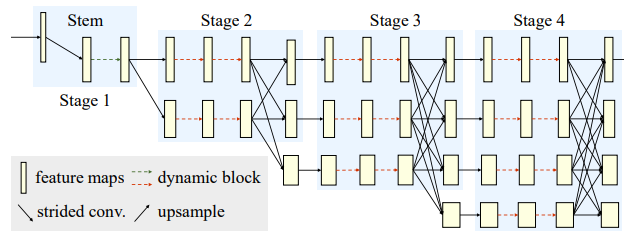
\includegraphics[scale = 0.7]{1}
		\caption{整体网络结构}
		\label{h}
\end{figure}
	\begin{multicols}{2}
		第一个阶段也称为Stem,包含一个$3\times3$的跨卷积和一个主分支上的动态全局上下文(DGC)块。每个后续阶段由一系列交叉解析模块组成,这些模块由两个动态多尺度上下文组成(DMC)块和跨所有分支交换信息的多尺度融合层。分辨率最高的主分支保持高分辨率表示,为后续的人体姿态估计提供骨干网的最终输出。
		\begin{figure}[H]
			\centering
			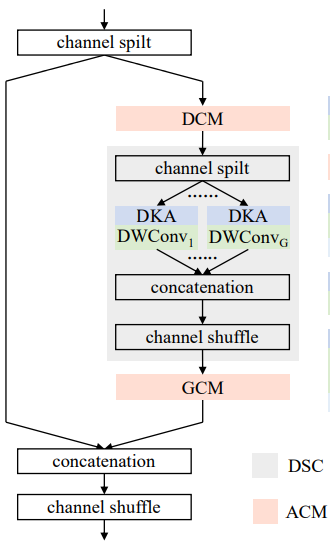
\includegraphics[scale = 0.45]{2}
			\caption{动态多尺度上下文块的结构}
			\label{a}
		\end{figure}
	
	图\ref{a}方法中将动态分裂卷积(Dynamic Split Convolution, DSC)应用于动态内核聚合(Dynamic Kernel Aggregation, DKA)DMC块和DGC块中的每个卷积。DCM(密集上下文建模)和GCM(全局上下文建模)是我们提出的自适应上下文建模(ACM)的两个实例。
	
	DMC块对一半图片通道应用层序列,而DGC块对所有两组通道应用两种不同的层序列。DMC块中的层序列包含一个
	密集上下文建模(DCM)操作,一个DSC和一个全球上下文建模(GCM)。DCM和GCM都是ACM方法的实例。
		\begin{figure}[H]
			\centering
			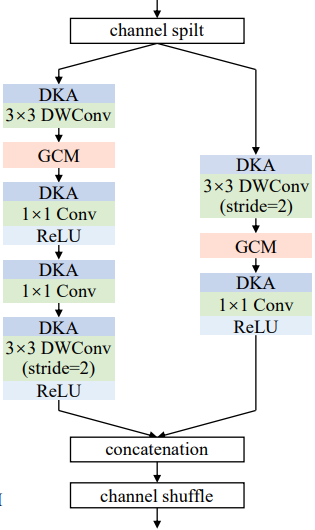
\includegraphics[scale = 0.45]{3}
			\caption{动态全局上下文块的结构}
			\label{b}
		\end{figure}
	在DGC块中(如图\ref{b}),一个$3\times3$阶深度卷积,一个GCM和一个在一组信道上进行$1\times1$卷积,在另一组信道上分别进行$3\times3$深度卷积、GCM卷积、$1\times1$卷积和$3\times3$跨步深度卷积。DGC块和DSC层的每一次卷积都通过动态内核聚合(Dynamic kernel Aggregation, DKA)生成卷积内核。
	\subsection{自适应上下文建模(ACM)}
	ACM方法可以抽象为以下三个步骤:(a)自适应上下文池化,通过$1\times1$的信道池化卷积和softmax层建立快捷连接,形成上下文掩码,然后通过一系列分辨率自适应变换将掩码应用到特征映射上,获得空间上下文特征;(b)上下文移位,通过两个$1\times1$卷积和非线性激活将空间相关的上下文特征重新组合在一起;(c)上下文加权,采用对应元素加权相加操作。上下文加权(Context weighted),是指在输入特征和移位的上下文特征之间进行元素加权运算,对对应特征的上下文关系进行建模。
	
	ACM方法的这种抽象可以定义为:
	$$Y = Weight(X, Shift(ACPool(H,W)(X)))$$
	
	其中$ACPool(H,W)(X)$表示自适应上下文池,将输入特征$X$池到特定的输出大小$H\times W$,$Shift(.)$表示上下文移动,$ Weight(.)$表示上下文权重。
	对于高分辨率网络,我们提出了ACM方法的两个实例,DCM和GCM,它们利用了并行多分辨率架构的优势。
	\subsection{密集上下文建模(DCM)}
	我们引入DCM操作来密集建模一个阶段所有分辨率分支的特征的空间上下文关系。在第n阶段,将所有n个分支的输入特征汇聚到分辨率最低的$H_n\times W_n$。然后,所有汇集的特性被连接在一起,这样就可以在并行的上下文特性上密集地执行上下文转移最后,将移位后的上下文特征上采样到相应的分辨率,并分布回相应的分支进行后续的上下文加权。
	这个实例化实现ACM如下:
	$$\left\{\begin{array}{l}
		\hat{X_k} = ACPool(H_n, W_n)(X_k)\\
		\tilde{X} = Shift(Cat([\hat{X}_1,...,\hat{X}_n]))\\
		Y_k = \left\{\begin{array}{l}
		Weight(X_k, Upsamp(\tilde{X_k})), 1\leq k\leq n-1\\
		Weight(X_k, \tilde{X_k}), \qquad k=n
		\end{array}\right.
	\end{array}\right.$$

	其中$Cat(.)$和$Upsamp(.)$分别表示特征拼接和上采样。$X_k$表示具有$k^{th}$最高分辨率的输入张量。$\hat{X}$表示来自$k^{th}$分支的集合张量。$\hat{X_k}$表示移位的张量,它被分配到$k^{th}$分支,即$\hat{X_k}$。$Y_k$表示对应的$k^{th}$输出张量。
	\subsection{动态内核聚合(DKA)}
	为了使SCS模块在卷积核很小的情况下也能学习到丰富的上下文信息,我们引入了一种DKA操作,通过基于输入图像的核关注权动态聚合多个核,增强了卷积核的输入依赖性。
	
	标准卷积核由4维权矩阵w定义,权矩阵w分别决定核大小和输入输出通道。我们没有将不同卷积的输出特征串联起来,而是在计算卷积结果之前将核权矩阵${w_i}$聚合起来,针对不同的输入动态生成不同的卷积核。DKA运算计算不同卷积核上的注意权值,然后将元素加权乘积应用于注意权值和核权值。我们如下定义DKA操作:
	
	$$Y = W^T(X)X$$
	$$W(X) = \sum_{i}^{N}a_i(X)w_i$$
	
	其中$a_i(X)$为$i^{th}$卷积核的注意权值,$W(X)$为N个卷积核的聚合权值矩阵。
	
	输入依赖注意权重$a(X)$由输入$X$计算如下:
	$$a(X) = Sigmoid(FC(ReLU(FC(GAP(X)))))$$
	
	其中$GAP(.)$表示全局平均池,$FC(.)$表示全连接层。两个函数$Sigmoid(.)$和$ReLU(.)$在两个完全连接的层之后用于非线性激活。
	
	由于DKA操作发生在计算卷积结果之前,因此聚合后的核对每个输入特征图只进行一次卷积操作,不会扩大网络宽度。
	
	为了在每个分辨率上分别建模全球空间依赖性,我们在网络的每个分支上应用GCM操作。当自适应上下文池的输出大小为$1 \times1$时,它是ACM的一个实例化。
	$$Y = Weight(X, Shift(ACPool(1,1)(X))) 1\leq k \leq n$$
	
	GCM操作在包含丰富上下文信息的全局面中捕获具有相同分辨率的所有特征的空间关系,而DCM操作在包含更多像素信息的中等面中捕获不同分辨率的所有特征的空间关系。
	
	同时,这两种操作都增加了跨特性的信息交换,因此可以更好地替代shuffle块中的$1\times1$卷积,而不是Lite-HRNet\cite{DBLP:journals/corr/abs-2109-15099}中的信道加权操作。
	
	\section{不足和改进}
	轻量级模型的发展使得神经网络更加高效, 从而能够广泛地应用到各种场景任务中.一方面, 轻量级神经网络有更小的体积和计算量, 降低了对设备存储能力和计算能力的需求, 既可以装配到传统家电中使其更加智能化, 也可以将深度学习系统应用在虚拟现实、增强现实、智能安防和智能可穿戴设备等新兴技术中; 另一方面, 轻量级神经网络具有更快的运行速度和更短的延时, 能够对任务进行实时处理, 对于在线学习、增量学习和分布式学习有重大意义; 另外, 实时处理的神经网络能够满足自动驾驶技术的需求, 提高自动驾驶的安全性.轻量级神经网络将对于人工智能技术的普及、建立智能化城市起不可或缺的作用
	
	目前的深度学习网络模型只能针对某一特定或同一类型的数据集,实现特殊的邻域任务。如何使用跨不同数据集的知识来加速优化过程, 是未来研究的热点。其他的挑战是联合优化深度神经网络流程的所有模型参数。到目前为止, 深度神经网络的通用自动化仍处于起步阶段, 许多问题尚未得到解决。然而, 这仍然是一个令人兴奋的领域, 并且未来的工作的方向需要强调其突出的实用性。
	
	为了提高整体网络结构对于特征图信息的学习能力,而注意机制在深卷积神经网络(DCNN)已经成为流行推动特征图信息中远程依赖关系,特定于像素级别的关注。可后续将目前泛化性较好的注意力机制模块加入进整体的网络模型中,在较小的损失速度的情况下,能够大幅度的提升精度。在整体网络结构的尾部采用PP-PicoDet\cite{DBLP:journals/corr/abs-2111-00902}提出了CSP-PAN结构,使用$1×1$的卷积将特征的通道数与 BackBone 输出的最小通道数进行统一,从而减少计算量,并保证特征融合性能不受影响。
	\end{multicols}
%		\section{单人姿态检测方法}
%		在给定人体位置的条件下,单人法估计人体在图像或视频中的姿态。一般情况下,在进行估计之前,先提供一个人的位置和大致的比例尺或一个人的边界框。早期的作品将人体部位建模为火柴棍(图\ref{e}),但最近的作品将其建模为关键关节,因为这些关节自然连接,。
%		(2)另一种算法首先生成热图,通过热图推断关键点位置。我们称之为基于热图的框架。
%		
%		\subsection{基于直接回归的框架}
%		有几篇文章是基于直接回归框架的。Toshev和Szegedy\cite{toshev2014deeppose}提出了级联反应DNN回归因子直接预测人类关键点。然而,如果没有其他的过程,从特征图中直接学习映射是很困难的。carira等人\cite{carreira2016human}使用了自校正模型。通过反馈误差预测,逐步优化预测的关键点位置。Sun等人\cite{sun2017compositional}提出了一种结构感知方法,称为“组合姿态回归”。与其他相关工作不同,这种方法使用骨骼而不是关节重新参数化姿态表示,更原始、更稳定、更容易学习。骨骼之间的长期相互作用由成分损失函数编码。Luvizon等人\cite{luvizon2019human}提出Soft-argmax以完全可微的方式将热图转换为坐标。采用基于关键点误差距离的损失函数和基于上下文的结构进行端到端可训练网络,使其能够实现与最先进的基于热图的框架相比较的结果。
%		\subsection{基于热力图的框架}
%		如图\ref{f}所示,许多文章都采用了基于热图的框架。一些文章在他们的模型中利用了人类的先验知识。例如Chen和Yuille\cite{chen2014articulated}使用的是DCNN学习到的成对关系的图形模型(零件类型和成对零件关系)。在另一项研究中,Chen et al.\cite{chen2017adversarial}采用条件生成的训练策略,融合了人体的先验敌对的网络(GANs)\cite{goodfellow2014generative}。
%		
%		网络结构设计一直是基于深度学习方法的一个主题。卷积的姿势机器(CPM)\cite{wei2016convolutional}在多个阶段回归热图,并使用中间监督来避免消失梯度。Newell等人\cite{newell2016stacked}设计了一种新的网络结构,称为“堆叠沙漏”。重复的自底而上,自顶而下的处理与中间监督被证明是提高人体姿态检测性能的关键。Chu等人\cite{chu2017multi}基于堆叠沙漏建立了他们的基线模型。他们采用了一种多情境注意机制,使模型更稳健、更准确。他们还通过耦合沙漏剩余单元来改进堆叠沙漏的结构。
%		
%		二维和三维之间的关系(3D)关键点检测也进行了探讨。Martinez等人\cite{martinez2017simple}提出利用深度神经网络直接利用2D关键点预测3D关键点。实验结果表明,二维检测是造成人体三维姿态估计误差的主要原因之一。
%		\subsection{讨论}
%		基于直接回归的框架和基于热图的框架,哪个框架更好?早期的文章\cite{toshev2014deeppose}\cite{pfister2014deep}和近期的一些文章\cite{chen2017adversarial}\cite{goodfellow2014generative}都尝试直接回归关键点的坐标。关节位置的直接回归是高度非线性的,在映射学习上存在困难\cite{tompson2014joint}\cite{pfister2015flowing}。此外,它不能应用于多人案件(自底向上方法或单个检测框包含一个以上的人)。相比之下,基于热图的框架首先回归热图。热图可以可视化,以增强人类的理解和模拟更复杂的情况。但是,如果将这些特定的技术结合起来\cite{chen2017adversarial},直接回归会更可靠,也有一些优点。当应用直接回归时,最终结果可以在不处理热图的情况下以端到端的方式获得。而且,它可以应用于3D场景,不需要太多的变化。此外,预测结果的精度依赖于热图分辨率,这需要较高的内存消耗。因此,对于这个问题没有一个绝对的结论,每个框架都有其优点和缺点。
%	\end{multicols}
%		
%		
%		
%		\begin{multicols}{2}
%		\section{多人姿态检测方法}
%		与单人检测方法相比,多人检测方法更困难,因为没有给出人员数量和位置信息。
%		关键点检测和人的定位是该任务的两个核心问题。为了解决这两个问题,目前比较流行的方法有:(1)自顶而下方法和(2)自底而上方法。
%		\subsection{自顶向下方法}
%		自顶向下方法的第一步是检测给定图像中的所有人,然后在每个检测到的边界框中执行单个人的方法。图\ref{g}显示了自顶向下方法的说明。除了人的检测,自顶向下的方法有更多的过程,可能会利用整个图像的上下文信息。示例如图。
%		
%		
%		Toshev和Szegedy\cite{toshev2014deeppose}利用FLIC数据集\cite{sapp2013modec}提出了第一种基于深度学习的自顶向下方法。人体姿态估计是回归研究中的一个关键问题。首先利用基于人脸的身体检测器估计人体的大致位置,然后采用基于多级级联DNN的关节坐标回归算子直接回归关节坐标。在之前的工作\cite{radosavovic2018data}中探讨了数据增强。Radosavovic等人\cite{radosavovic2018data}利用全监督学习,利用所有可用的数据(有标记的和无标记的)来训练模型。这项工作证明,最先进的人体姿势探测器足够准确,可以应用自我训练技术来挑战现实世界的数据。
%		
%		有些研究者研究了人体检测和人体盒子对准问题。Fang等人\cite{fang2017rmpe}注意到,单人姿势估计对人体检测很敏感。为了解决这个问题,他们采用了对称空间变压器网络(SSTN)与平行的单人姿态估计(SPPE)提取高质量的单人区域。Mask R-CNN\cite{he2017mask}同时预测人的包围盒和人的关键点,通过共享ConvNet的特征使检测速度更快。此外,RoI对齐可以实现更精确的特征图裁剪方法。这项工作没有结合人类骨骼的先验。加入人类骨骼的先验信息可能会进一步提高Make R-CNN的准确性。
%		
%		还有一些研究集中在人体检测框内的关键点估计。例如,Iqbal和Gall\cite{iqbal2016multi}认为多人姿态估计是一个关节对人的关联问题。他们的方法的目的是解决遮挡问题。通过局部关联检测到的关键点,消除了同一检测框中多余的人员部件。这项工作基于\cite{martinez2017simple},但是通过导入本地关联的机制执行得更快。Papandreou等人\cite{DBLP:journals/corr/PapandreouZKTTB17}提出了一种同时预测联合密集热图和位置偏移量的方法,将这两种输出集合起来,得到高度局域化的关键点位置。Chen等\cite{chen2018cascaded}提出了一种被称为级联金字塔网络的网络结构,它由两部分组成:GlobalNet和RefineNet。前者可以捕捉到良好的特征表示,而后者被用来处理准确例子。
%		
%		后处理方法已经在\cite{fang2017rmpe}中提出。数据驱动姿势非最大抑制在\cite{fang2017rmpe}中提出了(NMS)来解决遮挡问题,并使用姿态引导的提议生成器来进行数据增强。然而,严重的遮挡或误检仍然是该方法的一大挑战。\cite{DBLP:journals/corr/PapandreouZKTTB17}采用位姿评分和基于位姿的NMS方法消除假阳性,保持真阳性。
%		\subsection{关于自顶向下方法的讨论}
%		在自上而下的人体姿态估计中,人体探测器是否重要?自顶向下方法的第一步是人体检测。在人体姿态估计中最常用的人体探测器是基于Faster R-CNN结构的,因为它是一种高性能的现成检测器。更快的R-CNN有许多不同的基本网络(VGG\cite{simonyan2014very}, ResNet\cite{he2016deep},和
%		Inception- ResNet\cite{szegedy2017inception})和不同的扩展结构红外系统\cite{8099589})。这些变体具有不同程度的准确性、推断时间和计算复杂度。一般情况下,检测结果越准确,认为网络越复杂。因此,需要考虑准确性、消耗的内存和时间之间的权衡。
%		
%		一些工作比较了不同的人体检测器对人体姿态估计器的性能\cite{chen2018cascaded}。大多数工作结果表明,人体姿态估计的精度随着人体检测器的改进而提高。与此同时,在检测器性能较低的情况下,人体姿态估计器从性能较好的人体检测器获得较大增益。随着人体探测器平均精度的提高(AP),人体姿态估计器的AP增长较慢。当人体探测器达到非常高的精度(许多高性能人体探测器的集合)时,其人体姿态估计网络的精度将无法再提高。可能的原因是,没有被人类检测器检测到的人也是人类姿态估计器的困难例子。
%		
%		换句话说,人体探测器在性能一般的时候很重要,但在已经达到高性能的时候就不重要了。当人体检测AP较高时,姿态估计器的增益很小,特别是当人体检测器已经足够准确时。
%		
%		非极大值抑制是抑制冗余检测的常用方法。该技术可应用于自顶向下人体姿态估计方法的两个阶段。对于人类检测,有两种基础方式:标准抑制方式和软抑制方式\cite{bodla1704improving}。软抑制方式降低了检测框评分,标准抑制方式对检测框评分。软抑制方式在\cite{chen2018cascaded}中性能更好,但计算复杂度与标准抑制方式相同,使其成为一种简单的提高人体检测的方法。基于部分的非极大值抑制\cite{burgos2013merging}\cite{chen2015parsing}\cite{chen2014detect}可以消除同一检测框中的人体骨架实例。参考文献提出的方法。\cite{burgos2013merging}通过在标准坐标系中用质心替换中间点,将时间和空间上的部分合并非极大值抑制。但该方法仅适用于人体火柴杆模型。过去的一项研究\cite{chen2018cascaded}提出了一个基于非极大值抑制的OKS,它考虑了人类实例之间关键点的相似性。\cite{fang2017rmpe}中提出的参数位姿非极大值抑制是数据驱动的,即所有参数都是从数据中学习而不是手动设置。该方法比\cite{burgos2013merging}中提出的方法快得多,但比\cite{chen2018cascaded}中的非极大值抑制方法复杂。
%		\subsection{自底向上方法}
%		与自顶向下的方法相比,自底向上的方法有相反的过程,如图\ref{h}所示。在第一阶段检测所有的身体部位(关键点),然后在第二阶段将它们与人体实例关联。如图11所示。可以看到,自底向上方法的推断时间可能更快,因为它不需要分别检测每个人的姿势。示例如图\ref{j}。
%		
%		%\begin{figure}[H]
%		%	\centering
%		%	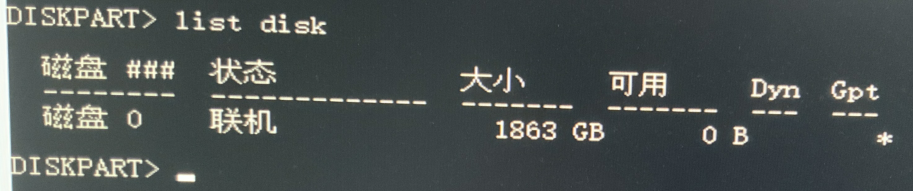
\includegraphics[scale = 0.7]{9}
%		%	\caption{自上而下方法框架}
%		%	\label{h}
%		%\end{figure}
%		
%		Pishchulin等人\cite{pishchulin2016deepcut}提出了第一种基于深度学习的自下而上姿态估计方法。它们的形成过程通过解决一个成本最低的多切割问题来执行估计任务,该问题将关键点的候选点建模为顶点,关键点的候选点之间的关系建模为边。
%		
%		Insafutdinov等人\cite{DBLP:conf/eccv/InsafutdinovPAA16}]对\cite{pishchulin2016deepcut}进行了三个方面的改进:(1)他们使用的网络比\cite{pishchulin2016deepcut}的网络更深入,产生了更有效的身体部位建议。(2)新的图像条件成对,使关键点建议组合成可变数量的人实例成为可能。(3)改变了优化策略,提高了精度和速度。尽管与之前的版本\cite{pishchulin2016deepcut}相比已经取得了显著的改进,但深度切割\cite{DBLP:conf/eccv/InsafutdinovPAA16}在解决最小成本、多切割问题时仍然很慢。参考文献\cite{8099625}提出的方法进一步改进了参考文献\cite{DBLP:conf/eccv/InsafutdinovPAA16}提出的方法,简化了整体-部分关系图,并将相当一部分计算量转移到前馈网络上。
%		
%		Cao等人\cite{DBLP:conf/cvpr/CaoSWS17}提出了一种有效的方法,该方法使用非参数表示,称为部分亲和性字段(PAFs)。在热图和PAFs生成后,利用贪心算法生成人体实例。Zhu et al.\cite{zhu2017multi}对\cite{DBLP:conf/cvpr/CaoSWS17}进行了多次修改,取得了更好的成绩。这些修改包括一个更深层的网络结构和新架构的PAFs,它们有助于将这些子连接连接到一个损坏的父连接上。
%		
%		同时,在\cite{newell2017associative}中提出了一种用于监督卷积神经网络检测和分组任务的关联嵌入方法。该方法可以同时预测局部热图和标记热图。标记热图的值对于同一个人是相似的,而对于不同的人是不同的。
%		\subsection{关于自底向上方法的讨论}
%		重点的位置是首先要考虑的,在人体姿态估计中,位置对算法的性能影响很大。在目前的工作中,有三种方法来生成地面真实热图。第一个是在每个关键点\cite{DBLP:conf/cvpr/CaoSWS17}处设置二维高斯激活的热图。第二种方法是将圆内以关键点为圆心,半径为R (hyper参数)的所有位置像素值设为1,其他位置设为0\cite{DBLP:journals/corr/PapandreouZKTTB17}\cite{DBLP:conf/eccv/InsafutdinovPAA16}。当使用这种类型的热图时,预测位置偏移图可以更准确地定位关键点。第三种方法是生成一个热的二进制掩模,其中只有一个像素被标记为前景。当使用一个热的热图时使用softmax损失,因为它们鼓励一个单点被检测到\cite{he2017mask}。热图的最大激活(或热图执行在一些著作中选择了高斯滤波器)作为重点\cite{zhu2017multi}。另一项研究\cite{DBLP:journals/corr/PapandreouZKTTB17}也使用热图来投票决定关键点的最终位置。
%		
%		检测关联是自底向上方法中的一个重要步骤。Deepcut\cite{pishchulin2016deepcut}只使用CNN来学习外观特征,使用其他手工定义的几何特征来拟合logistic模型进行两两概率估计。而Deepercut\cite{DBLP:conf/eccv/InsafutdinovPAA16}将人工计算的特征改变为深度神经网络生成的学习特征,极大地提高了AP。两种方法都采用了几何特征的逻辑模型来模拟关节的亲和度。同时学习PAFs\cite{zhu2017multi}和联合嵌入\cite{newell2017associative}。这两种方法的性能比\cite{pishchulin2016deepcut}中报告的性能要好。这是因为深度神经网络具有更大的容量,并直接从数据中学习,它可以捕捉局部特征和全局上下文。
%	\end{multicols}
%
%
%%\begin{figure}[H]
%%\centering
%%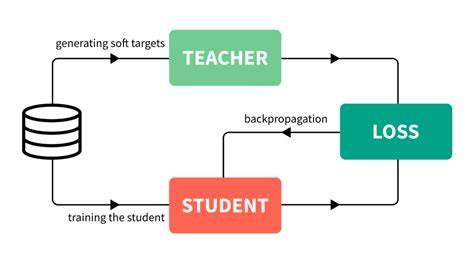
\includegraphics[scale = 0.33]{10}
%%\caption{自顶向下方法的示例。(a)输入图像,(b)人体检测器检测到两人,(c)裁剪后的单人图像,(d)单人姿态检测结果,(e)多人姿态检测结果。}
%%\label{i}
%%\end{figure}
%%\begin{figure}[H]
%%	\centering
%%	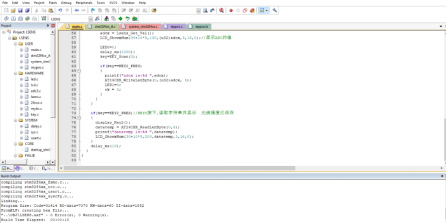
\includegraphics[scale = 0.36]{11}
%%	\caption{自底向上方法的示例。(a)输入图像,(b)所有人的关键点,(c)所有检测到的关键点连接起来,形成人的实例}
%%	\label{j}
%%\end{figure}
%\begin{multicols}{2}
%		\section{讨论}
%		相关的方法已经在上面进行了回顾,但没有详细讨论各方法的共同特点和差异。在本节中,将讨论一些关键过程(表\ref{table1}中列出),以揭示在这两种方法中什么是重要的。
%		\subsection{数据增强}
%		深度学习方法的性能高度依赖于数据输入。机器学习模型获得的数据越多,模型的有效性就越高。以往的研究大多利用数据增强来增强神经网络的泛化能力。用于人体姿态估计的简单而有效的数据增强技术包括裁剪、旋转、缩放和水平翻转输入图像。还有其他有前景的深度学习方法。使用未标记数据来训练网络是一个不发达的方向。数据蒸馏\cite{radosavovic2018data}是一种全监督学习方法,利用未标记数据进行数据增强。这一工作证明了相似和不同的未标记数据都是有用和有效的姿态估计。
%		\subsection{数据预处理}
%		数据集中的训练数据大小不一,使得网络很难从不均匀的数据中学习。为了使输入一致,图像总是在训练过程中调整大小。图像大小调整有两个重要因素:比例和绝对大小。在人体姿态估计任务中,人体检测盒被扩展到一个固定的比例,而不失真的图像,因为数据分布保持在这种方式。一个更大的训练图像总是可以为网络带来收益。一种可能的解释是,输入越大,分辨率越高,从而为网络提供更详细的信息。输入大小的比例也会影响训练结果。通常,调整后的图像的宽度和高度是相同的。然而,,宽度较短的输入图像AP值略有下降,因为数据集中大多数人的宽度都较短。大的输入图像在训练阶段占用更多的内存,同时能带来更好的增益。
%		\subsection{不同网络结构的比较}
%		网络设计是深度学习的基础工作。近年来针对分类任务提出了大量的网络结构\cite{xie2017aggregated}\cite{huang2017densely}。然后这些结构被转移到其他任务,如目标检测,图像分割和人体姿态估计。然而,这些网络不适合直接应用于人体姿态估计,因为需要更高分辨率的特征图来获得更精确的结果。为了解决这个问题,设计了两个结构来执行所需的过程。第一个是hole算法(也叫atrous convolution或dilation convolution)\cite{chen2017deeplab},它可以使各层在保持输出分辨率固定的同时有效地增加接收场。二是上采样,提高了输入特征图的特殊分辨率。后一种算法在分割任务时性能更好,但占用更多的GPU内存。这两种技术都在对图像进行裁剪时使用,得到合适的特征图大小。
%		
%		输出的步幅是另一个需要考虑的因素,因为在相同深度下,较小的步幅通常消耗更多的存储空间,但输出的热图分辨率更高。在之前的大部分作品中,最终的输出步幅都是8。在\cite{newell2017associative}中,步幅8网络已被证明可以取得与步幅4网络相似的结果。而\cite{newell2017associative}为单人姿态估计,在将检测结果发送到网络之前会调整大小,因此是否需要更小的步幅还在探索中。
%		
%		此外,与分类检测任务相比,人体姿态估计对关键点的位置更加敏感。为此,许多作品\cite{newell2017associative}\cite{zhu2017multi}都采用了浅层和深层之间的跳跃式连接。浅层由于分辨率高,包含更多的局部信息,而深层包含更多的语义信息。通过将本地信息和语义信息结合起来,跳过连接对这项任务有好处。
%		
%		有效接收野的大小也是设计良好网络的关键因素。接收野应该足够大,足以覆盖一个人的整个身体,这样所有的上下文信息都可以被包括在人体关键点检测中\cite{newell2017associative}\cite{zhu2017multi}。
%		
%		此外,Zhong等人\cite{zhong2018practical}提出了一种利用Q-learning自动设计高性能网络块的方法,应用于特定的人体姿态检测模块中。
%		\subsection{自顶向下与自底向上}
%		如前所述,近年来,深度学习方法已经探索了自底而上和自顶而下的方法。然而,哪种方法比另一种更好还有待确定,因为在实际应用程序中要考虑多个方面。精度和速度是多人姿态估计评价的两个关键因素。
%		
%		\textbf{准确度}:COCO 2017关键点的冠军\cite{DBLP:conf/cvpr/CaoSWS17}和AI挑战者Human的冠军\cite{chen2018cascaded}
%		骨骼系统关键点挑战采用了自顶向下的管道。而\cite{newell2017associative}报道自底而上的管道在融合多尺度结果进行测试时也能达到类似的精度。在考虑自底向上管道的情况下,人的尺度变化会给人体姿态估计带来困难,因为网络无法从图像中学习到一致的特征。另一个需要注意的事实是,输出特征图分辨率和网络容量是相互制约的。
%		
%		\textbf{速度}:自顶而下流水线中每个人的姿势是逐个估计的,随着人数的增加消耗线性时间。相反,在自底向上的管道中,图像只通过网络一次。当图像进行前向传播时,由于当前网络总是非常深,它总是需要更多的时间。但是,如果方法设计得当,分组时间可以非常短(9人分组时间为0.58 ms)。因此,在自底向上框架中更快的速度是可能实现的。
%		\subsection{人体姿态估计其他技巧}
%		大部分的技巧在上面都有说明,但是在最近的作品中还有其他的技巧。例如,在裁判中使用的中间监督。\cite{zhu2017multi}已经被证明在训练一个更好的网络是有效的,因为它迫使网络从较浅的层学习特征,并防止消失的梯度。
%		
%		多任务学习提高了模型在检测任务\cite{ren2015faster}和关键点检测任务中的性能,因为当任务相似时,网络可以学习到更强的特征表示。
%		
%		另一个技巧只适用于自底向上的管道。采用单人关键点检测模型对自底向上的网络模型进行改进,虽然降低了检测速度,但在精度上有了很大的提高。
%	\end{multicols}
%
%
%\begin{table}[H]
%	\centering
%	\caption{关键程序的列表}
%	\begin{tabular}{lllll}
%		\hline
%		关键程序                                      & \multicolumn{1}{c}{方法} & 单人      & 自顶向下    & 自底向上    \\ \hline
%		\multicolumn{1}{r}{\multirow{2}{*}{数据增强}} & 传统:裁剪、旋转、缩放和水平翻转       & $\surd$ & $\surd$ & $\surd$ \\ \cline{2-5} 
%		\multicolumn{1}{r}{}                      & 使用未标记数据:数据蒸馏           & $\surd$ & $\surd$ &         \\ \hline
%		数据预处理                                     & 不失真调整图片大小              & $\surd$ & $\surd$ & $\surd$ \\ \hline
%		\multirow{6}{*}{网络设计}                     & 上采样                  & $\surd$ & $\surd$ & $\surd$ \\
%		& 输出步幅\textless{}=8      &         &         &         \\
%		& 跳越连接                   &         &         &         \\
%		& 大的有效感受野                &         &         &         \\
%		& 自动搜寻法                  &         &         &         \\ \hline
%		\multirow{2}{*}{后处理}                      & 检测NMS                  &         & $\surd$ &         \\ \cline{2-5} 
%		& 骨架NMS                  &         & $\surd$ & $\surd$ \\ \hline
%	\end{tabular}
%	\label{table1}
%\end{table}
%
%	\begin{multicols}{2}
%		\section{指标和数据集}
%		\subsection{数据集}
%		人体姿态估计已被研究多年。然而,由于人体姿势各不相同,因此很难为这项任务创建一个通用的数据集。为了逐步解决估计问题,数据集的数量和复杂度都呈递增趋势。人体姿势数据集列表如表\ref{table2}所示和这些数据集的一些样本显示在图\ref{q}所示。早期的数据集包含背景相对简单的图像。然而,基于深度学习的方法并不适合这些数据集,因为图像数量太少,不适合训练。基于深度学习的方法中常用的数据集有MSCOCO\cite{lin2014microsoft}, MPII\cite{andriluka20142d}, LSP\cite{johnson2010clustered},FLIC\cite{sapp2013modec}, PoseTrack\cite{Andriluka2018PoseTrackAB}和AI Challenger\cite{Wu2017AIC}在更复杂的场景中包含更多的图像。LSP和FLIC数据集相对较小,只包含特定类别的活动。LSP数据集中的图像来自体育场景。FLIC数据集是从好莱坞电影中收集的。最新的数据集,如MSCOCO和AI Challenger在规模和类别数量上都更大。
%		
%		
%		\subsection{指标}
%		人体姿态估计的性能评估是一个困难的问题,因为需要考虑很多因素。在早期工作中使用的评估指标是正确估计的身体部位百分比(PCP)\cite{ferrari2008progressive},评估关键点预测结果。另一个广泛使用的关键点检测指标是PCK\cite{yang2011articulated}及其变体PCKh。在这两个指标中,一个指标是处于位于真实值关键点的周围$\alpha\cdot max(w,h)$像素,其中w和h是人的边界框的高度和宽度),另一个最近的指标包括目标关键点相似度(OKS)及其AP,该方法不仅考虑了规模,还引入了逐点常数来控制衰减。
%	\end{multicols}
%
%%\begin{figure}[H]
%%	\centering
%%	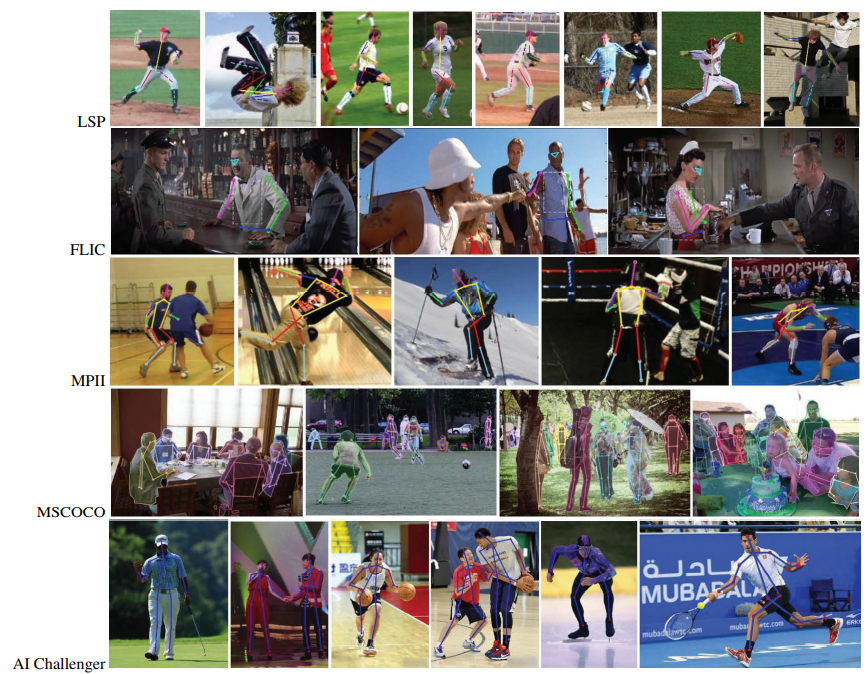
\includegraphics[scale = 0.5]{12}
%%	\caption{不同数据集的例子}
%%	\label{q}
%%\end{figure}
%
%\begin{table}[H]
%	\centering
%	\caption{人体姿态估计数据集}
%	\begin{tabular}{lllll}
%		\hline
%		年份                                        & \multicolumn{1}{c}{数据集}            & 大小              & 类型                   & 描述数量                    \\ \hline
%		\multicolumn{1}{c}{\multirow{2}{*}{2008}} & \multirow{2}{*}{Buffy}             & 472帧训练          & \multirow{2}{*}{上半身} & \multirow{2}{*}{6个身体部位} \\
%		\multicolumn{1}{c}{}                      &                                    & 276帧测试          &                      &                         \\ \hline
%		\multirow{2}{*}{2010}                     & \multirow{2}{*}{LSP}               & 1000张训练         & \multirow{2}{*}{全身}  & \multirow{2}{*}{14个关键点} \\
%		&                                    & 1000张测试         &                      &                         \\ \hline
%		\multirow{2}{*}{2013}                     & \multirow{2}{*}{FLIC}              & 3987张训练         & \multirow{2}{*}{上半身} & \multirow{2}{*}{10个关键点} \\
%		&                                    & 1016张测试         &                      &                         \\ \hline
%		\multirow{2}{*}{2014}                     & \multirow{2}{*}{Parse}             & 100张训练          & \multirow{2}{*}{全身}  & \multirow{2}{*}{14个关键点} \\
%		&                                    & 205张测试          &                      &                         \\ \hline
%		\multirow{2}{*}{2014}                     & \multirow{2}{*}{MPII Human pose}   & 410个活动          & \multirow{2}{*}{全身}  & \multirow{2}{*}{16个关键点} \\
%		&                                    & 25000张图片        &                      &                         \\ \hline
%		\multirow{2}{*}{2014}                     & \multirow{2}{*}{Poses in the wild} & 30个视频序列         & \multirow{2}{*}{上半身} & \multirow{2}{*}{5个关键点}  \\
%		&                                    & 900帧图片          &                      &                         \\ \hline
%		\multirow{3}{*}{2014}                     & \multirow{3}{*}{MSCOCO}            & 115000张图片训练     & \multirow{3}{*}{全身}  & \multirow{3}{*}{17个关键点} \\
%		&                                    & 5000张图片验证       &                      &                         \\
%		&                                    & 20000张图片测试实验    &                      &                         \\ \hline
%		\multirow{3}{*}{2017}                     & \multirow{3}{*}{AI Challenger}     & 210000张图片训练     & \multirow{3}{*}{全身}  & \multirow{3}{*}{14个关键点} \\
%		&                                    & 30000张图片验证      &                      &                         \\
%		&                                    & 60000张图片测试      &                      &                         \\ \hline
%		\multirow{4}{*}{2017}                     & \multirow{4}{*}{Pose Track}        & 514个视频包含66374帧图 & \multirow{4}{*}{全身}  & \multirow{4}{*}{15个关键点} \\
%		&                                    & 300个视频训练        &                      &                         \\
%		&                                    & 50个视频验证         &                      &                         \\
%		&                                    & 208个视频测试        &                      &                         \\ \hline
%	\end{tabular}
%	\label{table2}
%\end{table}



\newpage
%\nocite{*}


\bibliographystyle{cjc}
\bibliography{example}
\newpage


\textbf{附录}
\begin{Python}{DenseContextModeling}
class DenseContextModeling(nn.Module):
	def __init__(self, channels, reduction):
		super().__init__()
		num_branches = len(channels)
		self.reduction = reduction[num_branches-2]
		self.channels = channels
		total_channel = sum(channels)
		mid_channels = total_channel // self.reduction
		##这个是ACM中的adaptive context pooling, a context mask,一个1*1卷积和softmax部分 
		self.conv_mask = nn.ModuleList([
		nn.Conv2d(channels[i], 1, kernel_size=1, stride=1, padding=0, bias=True)
		for i in range(len(channels))
										])
		self.softmax = nn.Softmax(dim=2)

		##这个是shift操作——2个1*1卷积和一个sigmoid函数
		self.channel_attention = nn.Sequential(
			nn.Conv2d(total_channel, mid_channels, kernel_size=1, stride=1, padding=0, bias=False),
			nn.BatchNorm2d(mid_channels),
			nn.ReLU(inplace=True),
			nn.Conv2d(mid_channels, total_channel, kernel_size=1, stride=1, padding=0, bias=True),
			nn.Sigmoid()
			)
##这个就是真正的ACM实现
	def global_spatial_pool(self, x, mini_size, i):
		batch, channel, height, width = x.size()
		mini_height, mini_width = mini_size
		# [N, C, H, W]
		x_m = x
		# [N, C, H * W]
		x_m = x_m.view(batch, channel, height * width)
		# [N, MH * MW, C, (H * W) / (MH * MW)]
		x_m = x_m.view(batch, mini_height * mini_width, channel, (height * width) // (mini_height * mini_width))
		# [N, 1, H, W]
		mask = self.conv_mask[i](x)
		# [N, 1, H * W]
		mask = mask.view(batch, 1, height * width)
		# [N, 1, H * W]
		mask = self.softmax(mask)
		# [N, MH * MW, (H * W) / (MH * MW)]
		mask = mask.view(batch, mini_height * mini_width, (height * width) // (mini_height * mini_width))
		# [N, MH * MW, (H * W) / (MH * MW), 1]
		mask = mask.unsqueeze(-1)
		# [N, MH * MW, C, 1]
		x = torch.matmul(x_m, mask)
		# [N, C, MH * MW, 1]
		x = x.permute(0, 2, 1, 3)
		# [N, C, MH, MW]
		x = x.view(batch, channel, mini_height, mini_width)
		return x
	def forward(self, x):
		mini_size = x[-1].size()[-2:]
		out = [self.global_spatial_pool(s, mini_size, i) for s, i in zip(x[:-1], range(len(x)))] + [x[-1]]
		out = torch.cat(out, dim=1)
		out = self.channel_attention(out)
		out = torch.split(out, self.channels, dim=1)
		out = [s * F.interpolate(a, size=s.size()[-2:], mode='nearest') for s, a in zip(x, out)]
		return out
\end{Python}

\begin{Python}{GlobalContextModeling}
class GlobalContextModeling(nn.Module):
	def __init__(self, channels, num_branch, reduction, with_cp=False):
		super().__init__()
	
		self.with_cp = with_cp
	
		self.reduction = reduction[num_branch]
	
		mid_channels = channels // self.reduction
	
		self.conv_mask = nn.Conv2d(channels, 1, kernel_size=1, stride=1, padding=0, bias=True)
		self.softmax = nn.Softmax(dim=2)
	
		self.channel_attention = nn.Sequential(
			nn.Conv2d(channels, mid_channels, kernel_size=1, stride=1, padding=0, bias=False),
			nn.BatchNorm2d(mid_channels),
			nn.ReLU(inplace=True),
			nn.Conv2d(mid_channels, channels, kernel_size=1, stride=1, padding=0, bias=True),
			nn.Sigmoid()
			)
	
		self.bn = nn.BatchNorm2d(channels)
	
	def global_spatial_pool(self, x):
		batch, channel, height, width = x.size()
	
		# [N, C, H, W]
		x_m = x
		# [N, C, H * W]
		x_m = x_m.view(batch, channel, height * width)
		# [N, 1, C, H * W]
		x_m = x_m.unsqueeze(1)
		# [N, 1, H, W]
		mask = self.conv_mask(x)
		# [N, 1, H * W]
		mask = mask.view(batch, 1, height * width)
		# [N, 1, H * W]
		mask = self.softmax(mask)
		# [N, 1, H * W, 1]
		mask = mask.unsqueeze(-1)
		# [N, 1, C, 1]
		x = torch.matmul(x_m, mask)
		# [N, C, 1, 1]
		x = x.permute(0, 2, 1, 3)
		
		return x
	
	def forward(self, x):
	
		def _inner_forward(x):
			identity = x
			
			x = self.global_spatial_pool(x)
			x = self.channel_attention(x)
			x = self.bn(identity * x)
			
			return x
			
		if self.with_cp and x.requires_grad:
			x = cp.checkpoint(_inner_forward, x)
		else:
			x = _inner_forward(x)
				
			return x
\end{Python}
\begin{Python}{DynamicSplitConvolution}
class DynamicSplitConvolution(nn.Module):
	
	def __init__(self, channels, stride, num_branch, num_groups, num_kernels, with_cp=False):
		super().__init__()
		
		self.with_cp = with_cp
		
		self.num_groups = num_groups[num_branch]
		self.num_kernels = num_kernels[num_branch]
		
		self.split_channels = _split_channels(channels, self.num_groups)
		
		self.conv = nn.ModuleList([
		ConvBN(
		self.split_channels[i],
		self.split_channels[i],
		kernel_size=i * 2 + 3,
		stride=stride,
		padding=i + 1,
		groups=self.split_channels[i],
		num_kernels=self.num_kernels)
		for i in range(self.num_groups)
		])
		
		def forward(self, x):
		
			def _inner_forward(x):
			if self.num_groups == 1:
			x = self.conv[0](x)
			else:
			x_split = torch.split(x, self.split_channels, dim=1)
			x = [conv(t) for conv, t in zip(self.conv, x_split)]
			x = torch.cat(x, dim=1)
			x = channel_shuffle(x, self.num_groups)
			
			return x
			
			if self.with_cp and x.requires_grad:
				x = cp.checkpoint(_inner_forward, x)
			else:
				x = _inner_forward(x)
	
			return x
\end{Python}
\end{document}